%% Based on a TeXnicCenter-Template by Gyorgy SZEIDL.
%%%%%%%%%%%%%%%%%%%%%%%%%%%%%%%%%%%%%%%%%%%%%%%%%%%%%%%%%%%%%

%----------------------------------------------------------
%
%\documentclass{book}%
%
%----------------------------------------------------------
% This is a sample document for the standard LaTeX Book Class
% Class options
%       --  Body text point size:
%                        10pt (default), 11pt, 12pt
%       --  Paper size:  letterpaper (8.5x11 inch, default)
%                        a4paper, a5paper, b5paper,
%                        legalpaper, executivepaper
%       --  Orientation (portrait is the default):
%                        landscape
%       --  Printside:   oneside, twoside (default)
%       --  Quality:     final(default), draft
%       --  Title page:  titlepage, notitlepage
%       --  Columns:     onecolumn (default), twocolumn
%       --  Start chapter on left:
%                        openright(no, default), openany
%       --  Equation numbering (equation numbers on right is the default):
%                        leqno
%       --  Displayed equations (centered is the default):
%                        fleqn (flush left)
%       --  Open bibliography style (closed bibliography is the default):
%                        openbib
% For instance the command
          \documentclass[a4paper,12pt,reqno]{book}
% ensures that the paper size is a4, fonts are typeset at the size 12p
% and the equation numbers are on the right side.
%
\usepackage{amsmath}%
\usepackage{amsfonts}%
\usepackage{amssymb}%
\usepackage{graphicx}
%----------------------------------------------------------
\newtheorem{theorem}{Theorem}
\newtheorem{acknowledgement}[theorem]{Acknowledgement}
\newtheorem{algorithm}[theorem]{Algorithm}
\newtheorem{axiom}[theorem]{Axiom}
\newtheorem{case}[theorem]{Case}
\newtheorem{claim}[theorem]{Claim}
\newtheorem{conclusion}[theorem]{Conclusion}
\newtheorem{condition}[theorem]{Condition}
\newtheorem{conjecture}[theorem]{Conjecture}
\newtheorem{corollary}[theorem]{Corollary}
\newtheorem{criterion}[theorem]{Criterion}
\newtheorem{definition}[theorem]{Definition}
\newtheorem{example}[theorem]{Example}
\newtheorem{exercise}[theorem]{Exercise}
\newtheorem{lemma}[theorem]{Lemma}
\newtheorem{notation}[theorem]{Notation}
\newtheorem{problem}[theorem]{Problem}
\newtheorem{proposition}[theorem]{Proposition}
\newtheorem{remark}[theorem]{Remark}
\newtheorem{solution}[theorem]{Solution}
\newtheorem{summary}[theorem]{Summary}
\newenvironment{proof}[1][Proof]{\textbf{#1.} }{\ \rule{0.5em}{0.5em}}




\usepackage[ngerman,english]{babel}	
\usepackage{caption} %% for \captionof{}{}
%%%%%%%%%%%%%%%%%%%%%%%%%%%%%%%%%%%%%%%%%%%%%%%%%%%%%%%%%%%
%\usepackage{fancyhdr}
%\pagestyle{fancy}


% new koma package
\usepackage{scrpage2}
%%%%%%%%%%%%%%%%%%%%%%%%%%%%%%%%%%%%%%%%%%%%%%%%%%%%%%%%%%%%
% for koma headers
\pagestyle{scrheadings}
% define head and foot marks
\renewcommand{\chaptermark}[1]{\markboth{#1}{}}
\renewcommand{\sectionmark}[1]{\markright{-~#1}{}}
%\ihead{\leftmark}
\ihead{}					%left head
\chead{\leftmark} %right head
\ohead{} 					%right head
%\ohead{\pagemark}
\ifoot{}
\cfoot{}
\ofoot{}
\setheadsepline{.4pt}



%define paralle typeset
%%%%%%%%%%%%%%%%%%%%%%%%%%%%%%%%%%%%%%%%%%%%%%%%%%%%%%%%%%%%%%%%%%%%%%%%%%%
\usepackage{parallel} % 2003/04/13
\usepackage{pdfcolparcolumns} % 2008/08/11
\usepackage{blindtext}
\newcommand\LR[0]{}
\renewcommand\LR[2]{\begin{Parallel}[c]{0.475\textwidth}{0.475\textwidth}%
    \selectlanguage{ngerman}\ParallelLText{#1}%    
    \selectlanguage{english}\ParallelRText{#2}%    
    \ParallelPar%
    \end{Parallel}%
    }

%----------------------------------------------------------
\begin{document}

\frontmatter
\title{The Title of the Book}
\author{Author{s}}
\date{The Date}
\maketitle
\tableofcontents


%%%%%%%%%%%%%%%%%%%%%%%%%%%%%%%%%%%%%%%%%%%%%%%%%%%%%
\pagenumbering{arabic}

\ihead{}					%left head
\chead{\leftmark} %right head
\ohead{} 					%right head
%\ohead{\pagemark}
\ifoot{}
\cfoot{\pagemark}
\ofoot{}

%mainmatter

\chapter{Vorwort}
%Preface

%\LR{
		%\subsection{sub1 Parallel} 
%		\blindtext 
%		}{
		%\esubsection{sub2 Parallel}
%		 \blindtext
%}

\chapter{Personal}
%STAFF
%Emeritus
%Emrtitus
\section*{Emrtitus}
 
 \begin{minipage}[t]{\textwidth}
	\begingroup
	\parfillskip=0pt
	
  	\begin{minipage}[c]{0.25\textwidth}	
   		%\blindtext	
   		\centering
		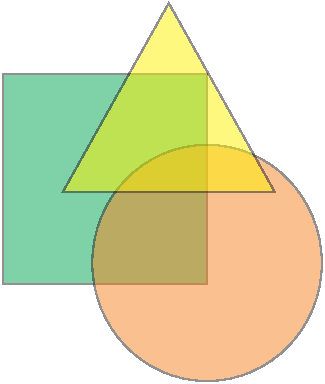
\includegraphics[width=0.7\textwidth]{Bilder/Grafik}		
		%\captionof{figure}{ Grafiken}	
			%\label{fig:GrafikOptionen}
  	\end{minipage}	
 	\hfill 	
  	\begin{minipage}[t]{0.7\textwidth}
  		\blindtext
  	\end{minipage}  
	\par\endgroup
\end{minipage}


% \begin{minipage}[t]{0.6\textwidth}
%	\begingroup
%	\parfillskip=0pt
%	% zwei weitere Minipages
%	\begin{minipage}[t]{0.47\textwidth}
%	\blindtext
%	\end{minipage}%
%	\hfill
%	\begin{minipage}[t]{0.47\textwidth}
%	\blindtext
%	\end{minipage}%
%	\par\endgroup
%\end{minipage}


%Technische Mitarbeiter und Sekretariat
%Technical staff and office
\newpage

\section*{Technische Mitarbeiter und Sekretariat}

\begin{figure}[htbp]
	% minipage mit (Blind-)Text
	\begin{minipage}[t]{0.18\textwidth} 
	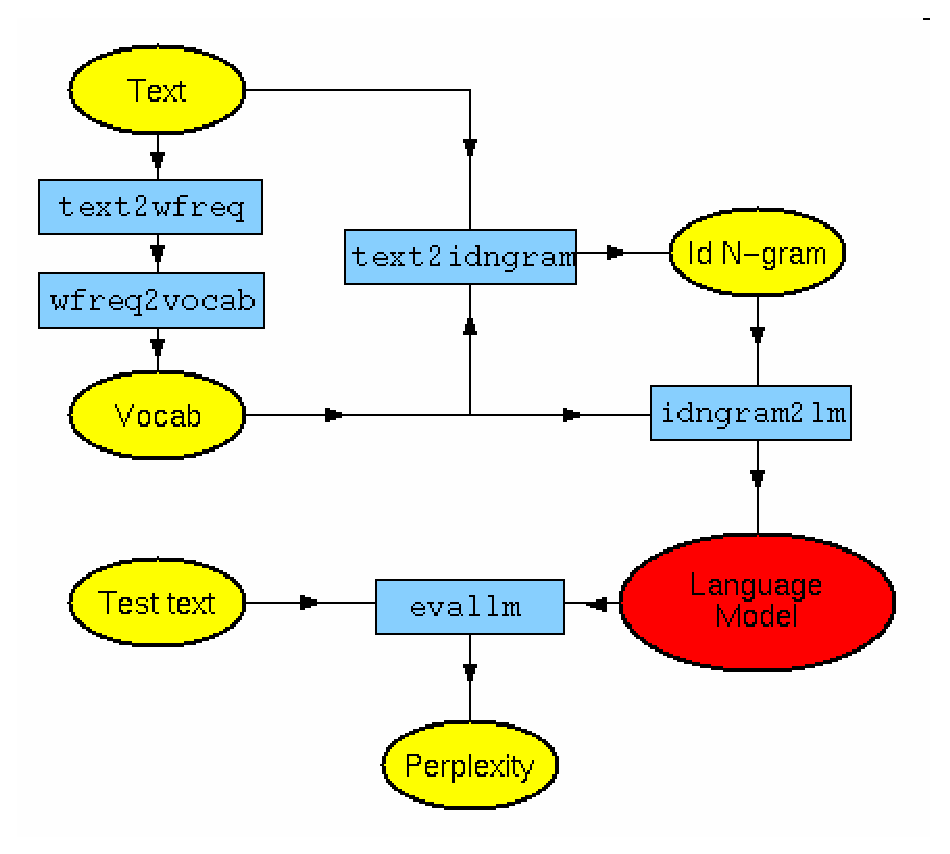
\includegraphics[width=\textwidth]{Bilder/toolkit.eps}
	%\caption{Eine Grafik}
	%\label{Bild}
	\end{minipage}
	% Auff�llen des Zwischenraums
	\hfill
	% minipage mit Grafik
	\begin{minipage}[b]{0.3\textwidth}
	% \textwidth bezieht sich nun auf die Minipage
 	\makebox[0.3\textwidth][l]{	\scriptsize{Dipl.-Ing Helmut Foth}	}\\
 	\makebox[0.3\textwidth][l]{	\scriptsize{Laboringenieur}	}\\
 	\makebox[0.3\textwidth][l]{	\scriptsize{Electrical engineering master}}\\
 	\makebox[0.3\textwidth][l]{	\scriptsize{Mitarbeit seit:1995}}\\		
 

 	
	% \caption{Der Text}
	% \label{Text}
	\end{minipage}
	\hfill
	% minipage mit (Blind-)Text
	\begin{minipage}[b]{0.18\textwidth} 
	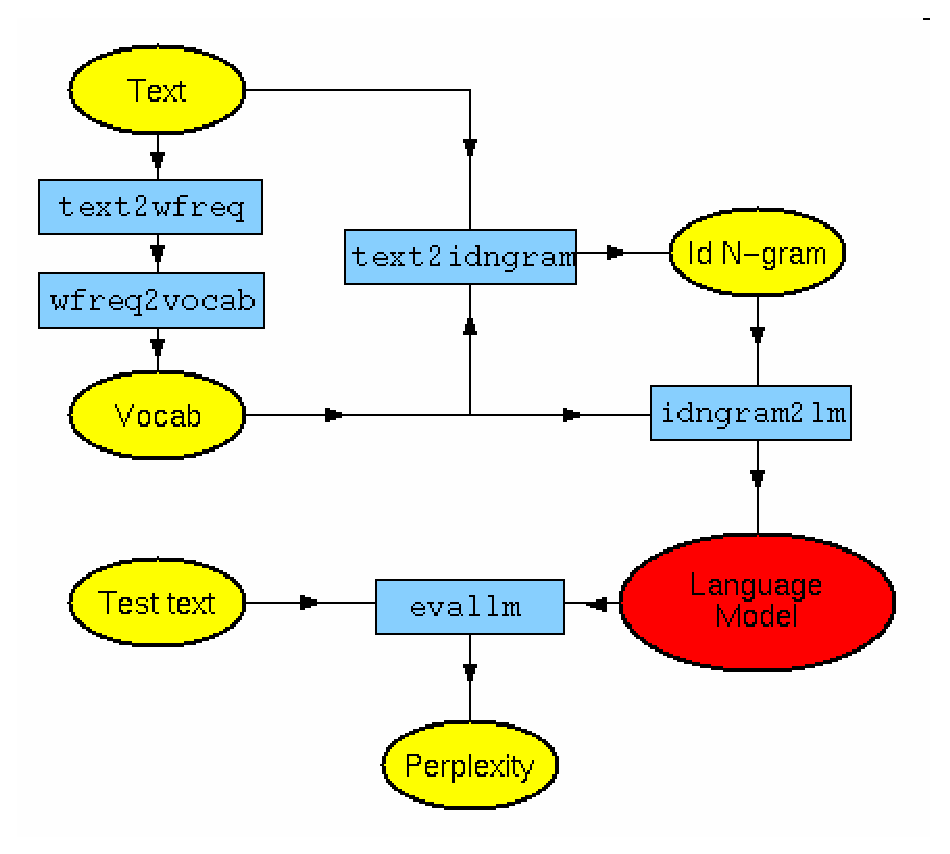
\includegraphics[width=\textwidth]{Bilder/toolkit.eps}
	%\caption{Eine Grafik}
	%\label{Bild}
	\end{minipage}
	% Auff�llen des Zwischenraums
	\hfill
	% minipage mit Grafik
	\begin{minipage}[b]{0.3\textwidth}
	% \textwidth bezieht sich nun auf die Minipage
 	\scriptsize{Title}\\
 	\parbox[b]{\textwidth}{
 	\scriptsize{Laboringenieur}	\\
 	\scriptsize{Electrical engineering technican}\\
 	\scriptsize{Mitarbeit seit:1995}\\	
 	}
	% \caption{Der Text}
	% \label{Text}
	\end{minipage}
% \caption{noch eine Caption}
\end{figure}


\begin{figure}[htbp]
	% minipage mit (Blind-)Text
	\begin{minipage}[b]{0.2\textwidth} 
	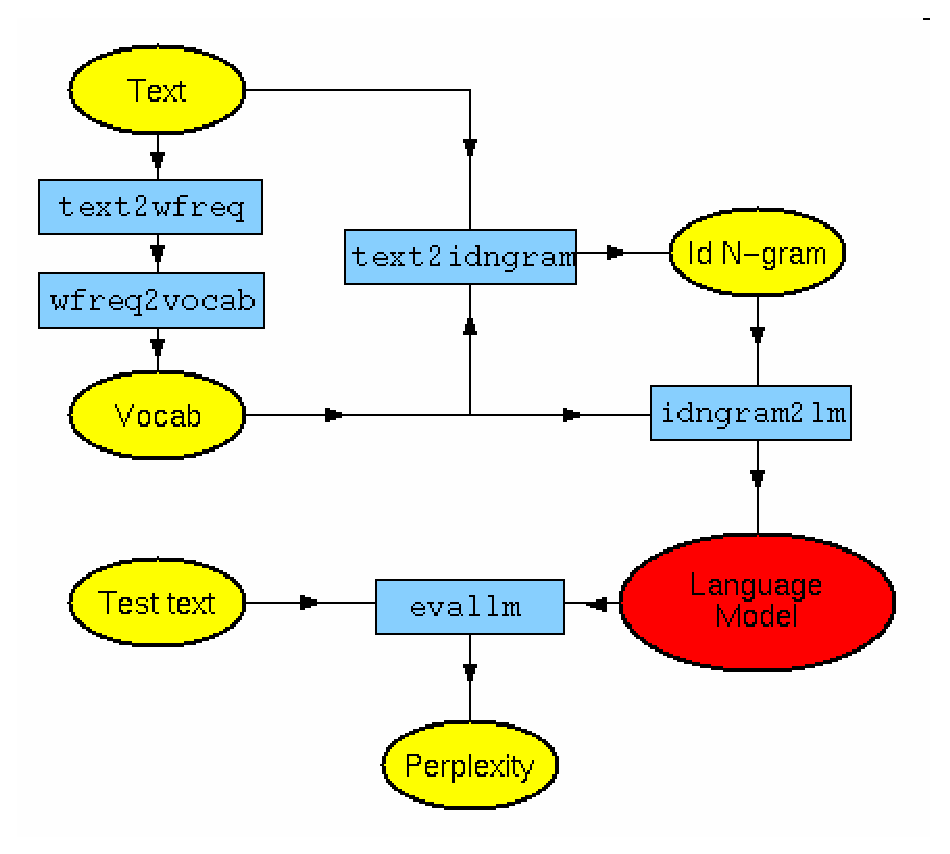
\includegraphics[width=\textwidth]{Bilder/toolkit.eps}
	%\caption{Eine Grafik}
	%\label{Bild}
	\end{minipage}
	% Auff�llen des Zwischenraums
	\hfill
	% minipage mit Grafik
	\begin{minipage}[b]{0.25\textwidth}
	% \textwidth bezieht sich nun auf die Minipage
 	Title\\
 	Job\\
 	Mitarbeit seit:1995\\	
	% \caption{Der Text}
	% \label{Text}
	\end{minipage}
	\hfill
	% minipage mit (Blind-)Text
	\begin{minipage}[b]{0.2\textwidth} 
	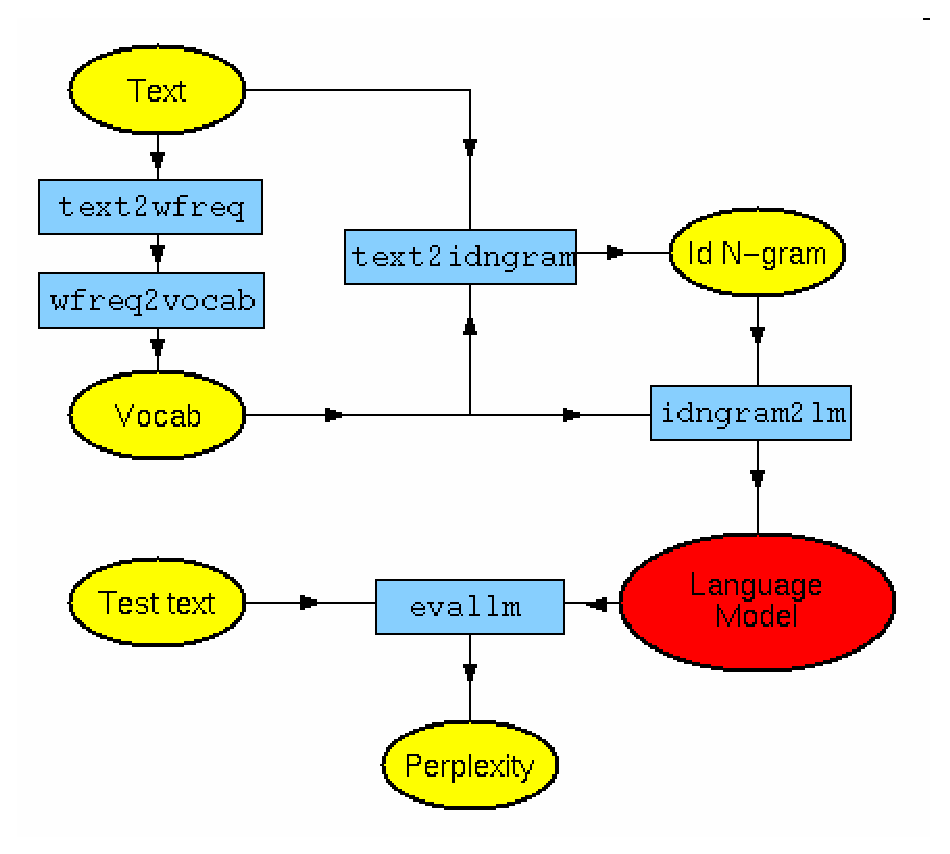
\includegraphics[width=\textwidth]{Bilder/toolkit.eps}
	%\caption{Eine Grafik}
	%\label{Bild}
	\end{minipage}
	% Auff�llen des Zwischenraums
	\hfill
	% minipage mit Grafik
	\begin{minipage}[b]{0.25\textwidth}
	% \textwidth bezieht sich nun auf die Minipage
 	Title\\
 	Job\\
 	Mitarbeit seit:1995\\	
	% \caption{Der Text}
	% \label{Text}
	\end{minipage}
% \caption{noch eine Caption}
\end{figure}

%Wissenschaftliche Mitarbeiter
%Scientific staff

\section*{Wissenschaftliche Mitarbeiter}


\chapter{Forschungsschwepunkte}

%\LR{
		%\subsection{sub1 Parallel} 
		%\blindtext \blindtext \blindtext \blindtext
%		}{
		%\esubsection{sub2 Parallel}
		% \blindtext \blindtext \blindtext \blindtext
%}

\chapter{Labor}


\chapter{Lehrveranstaltungen}


\chapter{Kooperationen}

%\include{sample}

\end{document}
